\documentclass[tikz,border=2pt]{standalone}

\usepackage{amsmath}
\usepackage{pifont}  % for \ding symbols
\usepackage{xcolor}
\usepackage{tikz}
\usetikzlibrary{arrows.meta,positioning,fit,backgrounds,calc,decorations.pathreplacing,patterns,shapes.geometric}
\usepackage{pgfplots}
\pgfplotsset{compat=1.18}
\usepgfplotslibrary{groupplots,fillbetween}

% ── Color palette (NeurIPS-style, colorblind-friendly) ──
\definecolor{bestcolor}{HTML}{E8F5E9}
\definecolor{gaincolor}{HTML}{1B5E20}
\definecolor{cStandard}{HTML}{BF616A}   % muted red
\definecolor{cAOI}{HTML}{5E81AC}        % steel blue
\definecolor{cDelta}{HTML}{A3BE8C}      % sage green
\definecolor{cVisual}{HTML}{D08770}     % muted orange
\definecolor{cASR}{HTML}{B48EAD}        % muted purple
\definecolor{cNarr}{HTML}{88C0D0}       % light blue
\definecolor{cAccent}{HTML}{EBCB8B}     % warm yellow
\definecolor{cGray}{HTML}{4C566A}       % dark gray
\definecolor{cLightGray}{HTML}{D8DEE9}  % light gray

\begin{document}

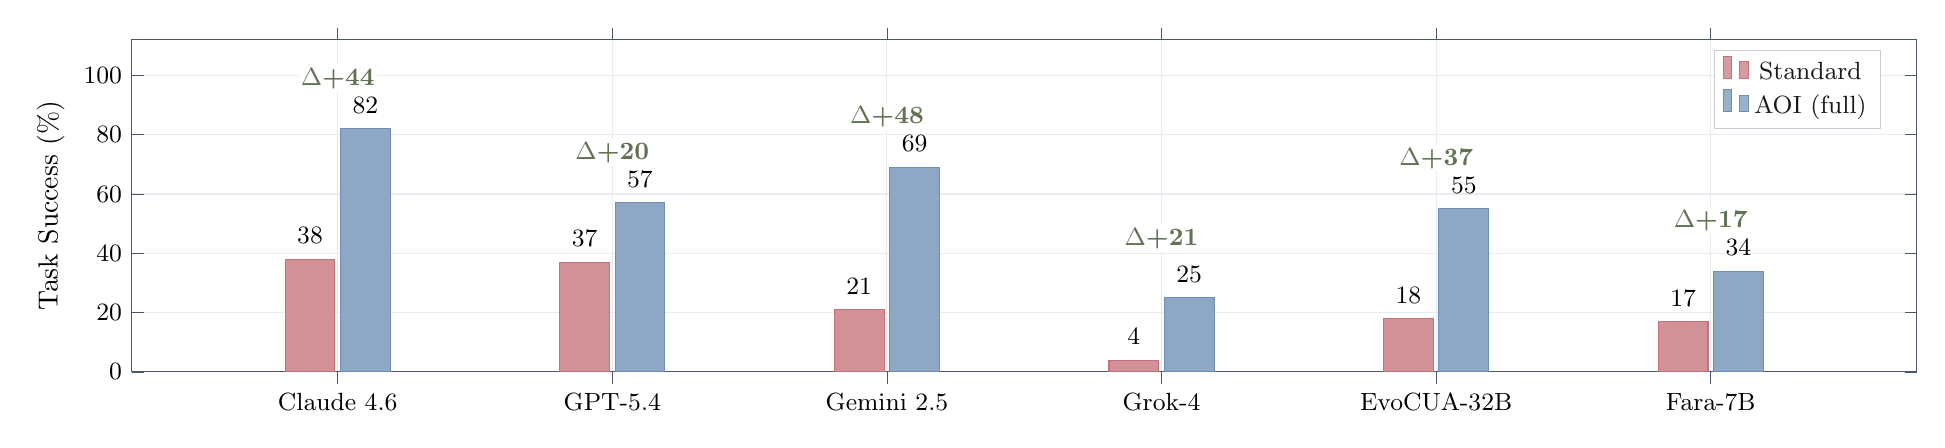
\begin{tikzpicture}
\begin{axis}[
    width=2\textwidth,
    height=5.8cm,
    ybar,
    bar width=18pt,
    ymin=0, ymax=112,
    ylabel={Task Success (\%)},
    ylabel style={font=\normalsize},
    symbolic x coords={Claude 4.6, GPT-5.4, Gemini 2.5, Grok-4, EvoCUA-32B, Fara-7B},
    xtick=data,
    xticklabel style={font=\small},
    ytick={0,20,40,60,80,100},
    yticklabel style={font=\small},
    legend style={at={(0.98,0.97)}, anchor=north east, font=\small,
                  draw=cGray!30, fill=white, fill opacity=0.9},
    grid=major,
    major grid style={cLightGray!60},
    axis line style={cGray},
    tick style={cGray},
    enlarge x limits=0.15,
    nodes near coords,
    nodes near coords style={font=\small\bfseries, /pgf/number format/fixed},
    every node near coord/.append style={above=2pt},
    clip=false,
]
% Standard bars
\addplot[fill=cStandard!70, draw=cStandard!90]
    coordinates {
      (Claude 4.6,    38)
      (GPT-5.4,       37)
      (Gemini 2.5,    21)
      (Grok-4,        4)
      (EvoCUA-32B,    18)
      (Fara-7B,       17)
    };
\addplot[fill=cAOI!70, draw=cAOI!90]
    coordinates {
      (Claude 4.6,    82)
      (GPT-5.4,       57)
      (Gemini 2.5,    69)
      (Grok-4,        25)
      (EvoCUA-32B,    55)
      (Fara-7B,       34)
    };
\legend{Standard, AOI (full)}

% Delta annotations — positioned well above AOI nodes near coords labels
\node[font=\small\bfseries, text=cDelta!60!black, fill=white, inner sep=1pt, rounded corners=1pt]
    at (axis cs:Claude 4.6, 99) {$\Delta$+44};
\node[font=\small\bfseries, text=cDelta!60!black, fill=white, inner sep=1pt, rounded corners=1pt]
    at (axis cs:GPT-5.4, 74) {$\Delta$+20};
\node[font=\small\bfseries, text=cDelta!60!black, fill=white, inner sep=1pt, rounded corners=1pt]
    at (axis cs:Gemini 2.5, 86) {$\Delta$+48};
\node[font=\small\bfseries, text=cDelta!60!black, fill=white, inner sep=1pt, rounded corners=1pt]
    at (axis cs:Grok-4, 45) {$\Delta$+21};
\node[font=\small\bfseries, text=cDelta!60!black, fill=white, inner sep=1pt, rounded corners=1pt]
    at (axis cs:EvoCUA-32B, 72) {$\Delta$+37};
\node[font=\small\bfseries, text=cDelta!60!black, fill=white, inner sep=1pt, rounded corners=1pt]
    at (axis cs:Fara-7B, 51) {$\Delta$+17};

\end{axis}
\end{tikzpicture}
\end{document}